\appendix
\section{Proofs}\label{app:proofs}

Throughout, $F$ has support $[0,\bar v]$ and positive density, and $G_{(2:m)}(y)=F(y)^m+mF(y)^{m-1}(1-F(y))$ is the probability that at most one of $m$ valuations exceeds $y$, i.e.\ the CDF of $v_{(2:m)}$.

\paragraph{Proof of Proposition~\ref{prop:veto}.} (i) For $m\ge2$, $\Pi(m,R)=\mathbb{E}[\max\{v_{(2:m)},R\}]=R+\int_R^{\bar v}\big(1-G_{(2:m)}(y)\big)\,dy$. Adding a bidder can only add values above $y$, so ``at most one of $m+1$ exceeds $y$'' implies ``at most one of the first $m$ exceeds $y$''. Hence
\begin{align*}
G_{(2:m)}(y)-G_{(2:m+1)}(y)&=\Pr(\text{exactly one of the first $m$ exceeds $y$, and so does the new one})\\
&= mF(y)^{m-1}(1-F(y))^2 ,
\end{align*}
which is strictly positive on $(0,\bar v)$. So $\Pi(m+1,R)-\Pi(m,R)=\int_R^{\bar v}mF^{m-1}(1-F)^2\,dy>0$ whenever $R<\bar v$. Monotonicity in $k$ follows from $m=N-k$.
(ii) The increment $\Delta(m)=\int_R^{\bar v}mF^{m-1}(1-F)^2dy$ tends to zero as $m\to\infty$ by dominated convergence, because $mF^{m-1}\to0$ pointwise on $F<1$. For $F=U[0,1]$ and $R=0$, $\mathbb{E}[v_{(2:m)}]=(m-1)/(m+1)$, so $\Delta(m)=2/((m+1)(m+2))$, which is strictly decreasing.
(iii) For $U[0,1]$ and $R=0$, $\Pi(1)=\beta\,\mathbb{E}[v]=\beta/2$ and $\Pi(2)=\mathbb{E}[\min(v_1,v_2)]=1/3$. Hence $\Pi(2)>\Pi(1)$ if and only if $\beta<2/3$. $\square$

\paragraph{Proof of Proposition~\ref{prop:audience}.} (i) For $m\ge2$, differentiating $R+\int_R^{\bar v}(1-G_{(2:m)})$ gives $1-(1-G_{(2:m)}(R))=G_{(2:m)}(R)>0$ for $R>0$. For $m=1$, $\Pi=R+\beta\int_R^{\bar v}(1-F)$, so $\partial\Pi/\partial R=1-\beta(1-F(R))>0$ when $\beta<1$ or $F(R)>0$. Because $R_{\text{pub}}<R_{\text{priv}}$ by (\ref{eq:R}) and $\lambda_{\text{pub}}<\lambda_{\text{priv}}$, $\Pi(m,R_{\text{pub}})<\Pi(m,R_{\text{priv}})$.
(ii) The loss from publicity is $L(m)=\int_{R_{\text{pub}}}^{R_{\text{priv}}}\partial\Pi/\partial R\,dr$. For $m\ge2$ the integrand $G_{(2:m)}(r)$ is strictly decreasing in $m$ by the argument in (i) above, so $L(m)$ is strictly decreasing. Comparing $m=1$ and $m=2$: $1-\beta(1-F)\ge 1-(1-F)^2=G_{(2:2)}$ if and only if $\beta\le 1-F$, which holds on $[R_{\text{pub}},R_{\text{priv}}]$ when $\beta\le 1-F(R_{\text{priv}})$. $\square$

\paragraph{Outside-option refinement.} In Rubinstein alternating offers between $T$ and a single acquirer with discount factors $\delta_T,\delta_A$, and with $T$ able to opt out to $R$ at any point, the unique subgame-perfect payoff to $T$ is $\max\{\beta^\ast v,R\}$, where $\beta^\ast=(1-\delta_A)/(1-\delta_T\delta_A)$ \citep{rubinstein1982,bss1989}. A fall in $R$ therefore changes $T$'s payoff only when $R>\beta^\ast v$.

\paragraph{Proof of the publicity condition (\ref{eq:public}).} $P$'s expected payoff from signal $s$ is $\tau_s u_{\text{out}}+(1-\tau_s)\big[u_{\text{stay}}-c_P\,\mathbf{1}\{s=\text{pub}\}\lambda_s\big]$, where the audience cost is paid only if he reconciles. The cost $c_P$ enters through $\lambda_{\text{pub}}$, the probability of the reconciliation that would trigger it; to a first approximation it is incurred with that probability. Rearranging the comparison gives (\ref{eq:public}). With $m\ge2$, $\tau_s=1-F(R_s)^m$, which is decreasing in $R_s$, so $\tau_{\text{pub}}>\tau_{\text{priv}}$. $\square$

\paragraph{Proof of Proposition~\ref{prop:delay}.} Selling now yields $\Pi(m,R)$. Waiting yields $V=1$ with probability $\rho$, and otherwise the discounted sale value $\delta\Pi(m',R')$. The comparison is immediate. Since $\Pi$ is increasing in $m$, a low current $m$ lowers the left-hand side of the sell-now comparison, and $m'>m$ raises the value of waiting. $\square$

\paragraph{Proof of Proposition~\ref{prop:price}.} Let $U_P=w+B(k)$ and $U_T=Y-w-C(k)$, with disagreement payoffs $\underline U_P,\underline U_T$. Generalised Nash bargaining with transferable utility gives $U_P-\underline U_P=\alpha S(k)$, where $S(k)=Y+B(k)-C(k)-\underline U_P-\underline U_T$. Solving, $w(k)=\underline U_P+\alpha S(k)-B(k)$, so $w(k)-w(0)=-(1-\alpha)B(k)-\alpha C(k)$ (normalising $B(0)=C(0)=0$). Then $\partial w/\partial k=-(1-\alpha)B'(k)-\alpha C'(k)$, and $C'(k)=q\,\partial[\Pi(N,R)-\Pi(N-k,R)]/\partial k+C_0'(k)$ rises with $q$ because $\Pi$ is increasing in $m$. If $w$ is constrained from below, the first-order condition for $k$ ($B'=C'$) holds with $C'$ increasing in $q$, so the chosen $k$ falls as $q$ rises. $\square$

\paragraph{Proof of Proposition~\ref{prop:informal}.} Approved acquirers value $P$ at $x_i+E>\bar x\ge x_j$ for every unapproved $j$. With $|A|\ge2$, the two highest valuations among all $N$ acquirers therefore both belong to $A$. The competitive price is the second-highest approved valuation, exactly as in a sale restricted to $A$. Because $x_i$ is increasing in the remaining term $\tau$, $\bar x(\tau)$ is increasing in $\tau$, so the condition $E>\bar x(\tau)$ is easier to satisfy near the end of a contract. $\square$

\section{Data Appendix}\label{app:data}

\paragraph{Sources.} Contracts and transactions: CapWages player pages (\url{https://capwages.com/players/*}), all 7,971 slugs in the site's sitemap, collected 30 October 2026; 7,965 returned data (script \path{analysis/02_fetch_capwages.py}). Rosters for coverage checks: NHL public API, \path{api-web.nhle.com/v1/roster/<team>/<season>} (script \path{01_fetch_rosters.py}). Salary cap: NHL CBA and league announcements (\path{data/salary_cap_by_season.csv}). The 2012--13 figure is the \$70.2 million full-season-equivalent limit rather than the nominal \$60 million. Deadline-day counts: NHL Stats Pack \citep{nhl_statspack}. Cases: news reports cited row by row in \texttt{data/protected\_player\_cases.csv}.

\paragraph{Key variables.}
\begin{description}[leftmargin=1em,itemsep=1pt,font=\normalfont\itshape]
\item[clause] The strongest protection listed for the contract-season: NMC $>$ M-NMC $>$ NTC $>$ M-NTC $>$ none.
\item[list\_n, list\_type] The first list size parsed from the clause text. ``block'' means a no-trade list (teams the player may refuse); ``approve'' means a trade list (teams he would accept). The parse is approximate where lists change by season.
\item[protected trade] A trade, identified by a CapWages trade ID, that moved at least one player whose contract carried any clause in that league year.
\item[star] A cap hit of at least 7.5 per cent of the upper limit in that season.
\item[deadline day] The February--April date with the most trades in the league year. It matches the official deadline date in every season from 2008--09 to 2025--26.
\item[pick value] Expected career NHL games by overall pick, from the 2005--14 drafts. A pick whose player never played, or is absent from the archive, counts as zero. Values are smoothed with $\hat g(p)=a(p+c)^{-b}+d$ and normalised to pick 16. Pick slots that are not yet known are set to 16 (first round), 48 (second), 80 (third), 112 (fourth) and 208 (seventh).
\item[realized\_gp\_3yr] Regular-season NHL games played by players received, in the league year of the trade and the two following.
\end{description}

\paragraph{Known gaps.} Coverage is incomplete before 2013--14 (Section~\ref{sec:empirics}). Pick-only trades are excluded from trade counts. Clause types are as reported by CapWages and were not independently audited contract by contract. Request dates in several cases are approximate, and the case file flags each one. See \texttt{METHODS\_NOTES.md} for the full list.

\begin{figure}[h]\centering
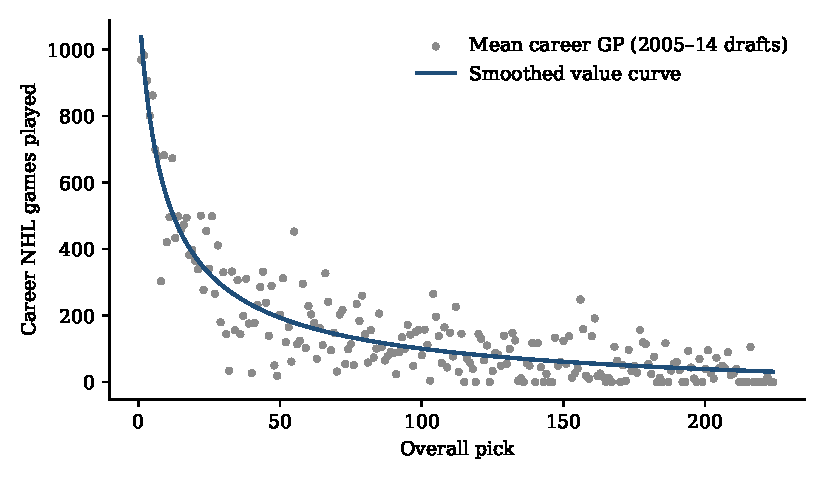
\includegraphics[width=0.7\linewidth]{../analysis/figures/pick_value.pdf}
\caption{Empirical draft-pick value chart: mean career NHL games by overall pick, 2005--14 drafts, with fitted curve.}\label{fig:pickvalue}
\end{figure}

\clearpage\section{Case Table}\label{app:cases}
\begin{table}[h]\centering\scriptsize
\caption{Star exits, demands and refusals, 2007--08 to 2026--27}\label{tab:cases}
\resizebox{\linewidth}{!}{\begin{tabular}{llllrrrrl}\toprule
Player & Team & Season & Clause & $m$ & Days & Picks & GP3 & Outcome\\\midrule
Mats Sundin & TOR & 2007-08 & NMC &  &  &  &  & stayed; signed with VAN as UFA\\
Dany Heatley & OTT & 2009-10 & NTC &  & 95 & 0.46 & 270 & SJS\\
Rick Nash & CBJ & 2011-12 & NMC & 4 & 185 & 1.00 & 395 & NYR\\
Jarome Iginla & CGY & 2012-13 & NTC &  &  & 0.70 & 24 & PIT\\
Martin St. Louis & TBL & 2013-14 & NMC & 1 & 49 & 2.00 & 215 & NYR\\
Roberto Luongo & VAN & 2013-14 & NTC & 1 & 678 & 0.00 & 278 & FLA\\
Ryan Kesler & VAN & 2013-14 & NTC & 2 & 132 & 1.07 & 362 & ANA\\
Jason Spezza & OTT & 2014-15 & M-NTC & 19 & 26 & 0.46 & 259 & DAL\\
Matt Duchene & COL & 2017-18 & none & 30 & 315 & 2.60 & 290 & OTT\\
Phil Kessel & PIT & 2018-19 & M-NTC &  & 45 & 0.00 & 181 & ARI\\
Pierre-Luc Dubois & CBJ & 2020-21 & none & 30 & 21 & 0.00 & 363 & WPG\\
Duncan Keith & CHI & 2021-22 & NMC &  & 27 & 0.29 & 149 & EDM\\
Jack Eichel & BUF & 2021-22 & none & 31 & 178 & 1.46 & 410 & VGK\\
Vladimir Tarasenko & STL & 2022-23 & NTC &  & 625 & 1.21 & 124 & NYR\\
Patrick Kane & CHI & 2022-23 & NMC & 2 &  & 0.67 & 0 & NYR\\
Erik Karlsson & SJS & 2023-24 & NMC &  & 52 & 1.00 & 399 & PIT\\
Patrik Laine & CBJ & 2024-25 & M-NTC & 21 & 65 & 0.00 &  & MTL\\
Seth Jones & CHI & 2024-25 & NTC &  & 19 & 1.00 &  & FLA\\
Mitch Marner & TOR & 2024-25 & NMC &  &  & 0.00 &  & VGK\\
Quinn Hughes & VAN & 2025-26 & none &  & 164 & 1.00 &  & MIN\\
Brady Tkachuk & OTT & 2025-26 & NMC & 4 & 51 & 3.57 &  & FLA\\
Dylan Larkin & DET & 2026-27 & NTC & 3 $\to$ 10 & 148+ &  &  & unresolved\\
Darnell Nurse & EDM & 2026-27 & NMC & 3 $\to$ 4 & 20 & 0.00 &  & SJS\\
Zach Werenski & CBJ & 2026-27 & NMC &  &  &  &  & stayed\\
Connor Hellebuyck & WPG & 2026-27 & NMC &  & 57 & 0.55 &  & NJD\\
\bottomrule\end{tabular}}
\begin{minipage}{0.97\linewidth}\footnotesize\vspace{4pt}
\emph{Notes:} $m$ is the reported number of approved destinations, where known. For Spezza and Laine it is computed from a ten-team no-trade list. Days run from the request, or from the public statement when the private date is unknown, to the trade; ``+'' marks a censored spell. Picks is incoming pick capital in mid-first-round equivalents. GP3 is the games played by incoming players over three seasons, shown for trades completed by 2023--24. Full sourcing, request types and conflicting accounts are recorded in \texttt{data/protected\_player\_cases.csv}.
\end{minipage}
\end{table}
